\begin{problem}[1.1]\leavevmode
  \begin{enumerate}
    \item For each of the three metrics in Example 1.4, sketch the open ball of some radius $r > 0$ around the origin in $\R^2$:
      \[%
        B_r(0) = \{(x, y) \in \R^2 \mid \metric{((x, y), 0)} < r\}
      .\]%

    \item For one of the three metrics (your choice), prove or give a counterexample to the following statement: a sequence of points $(x_1, y_1), (x_2, y_2), \cdots \in \R^2$ converges to a limit $(x, y)$ if and only if $x_n \to x$ and $y_n \to y$ separately, as sequences in $\R$ with the usual metric.

    \item Why is
      \[%
        \metric(\x, \y) = \min(\{|x_1 - y_1|, |x_2 - y_2|, \cdots, |x_n - y_n|\})
      ,\]%
      not a metric on $\R^n$?
  \end{enumerate}
\end{problem}

\begin{solution}[i]
  For the Euclidean metric, we have $\metric_2((x, y), (0, 0))$, we have
  \[%
    B_r^{(2)}(0) = \{(x, y) \in \R^2 \mid \sqrt{x^2 + y^2} < r\} = \{(x, y) \in \R^2 \mid x^2 + y^2 < r^2\}
  .\]%
  This is an open disk of radius $r$ centered ta the origin.

  For the taxicab metric, we have $\metric_1((x, y), (0, 0))$, we have
  \[%
    B_r^{(1)}(0) = \{(x, y) \in \R^2 \mid |x| + |y| < r\}
  .\]%
  This is the interior of a diamond (a square rotated by $45^\circ$) with vertices at $(r, 0)$, $(0, r)$, $(-r, 0)$, and $(0, -r)$.

  For the supremum metric, we have $\metric_\infty((x, y), (0, 0))$, we have
  \[%
    B_r^{(\infty)}(0) = \{(x, y) \in \R^2 \mid \max(|x|, |y|) < r\} = \{(x, y) \in \R^2 \mid |x| < r, |y| < r\}
  .\]%
  This is the interior of an axis-aligned square with vertices at $(r, r)$, $(-r, r)$, $(-r, -r)$, and $(r, -r)$.

  \begin{figure}[h]
    \centering

    \def\r{2}
    \begin{subfigure}[b]{0.45\textwidth}
      \centering

      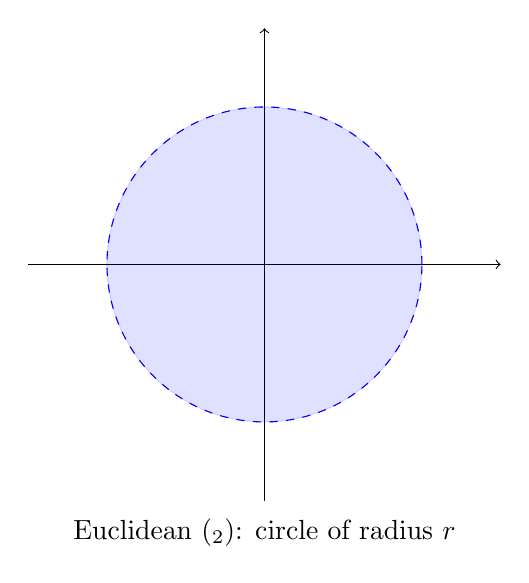
\begin{tikzpicture}[scale=1]
        % axes
        \draw[->] (-3,0) -- (3,0);
        \draw[->] (0,-3) -- (0,3);
        \draw[blue,fill=blue,opacity=0.12] (0,0) circle (\r);
        \draw[blue,dashed] (0,0) circle (\r);
        \node[below] at (0,-3.1) {Euclidean ($\metric_2$): circle of radius $r$};
      \end{tikzpicture}
    \end{subfigure}
    \begin{subfigure}[b]{0.45\textwidth}
      \centering

      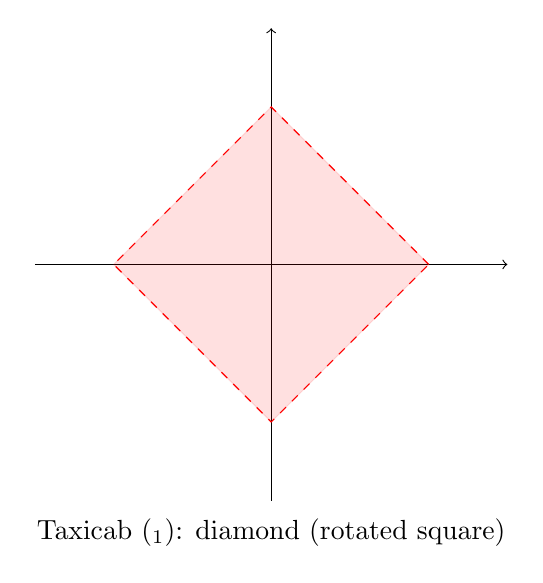
\begin{tikzpicture}[scale=1]
        \draw[->] (-3,0) -- (3,0);
        \draw[->] (0,-3) -- (0,3);
        \draw[red,fill=red,opacity=0.12] (\r,0) -- (0,\r) -- (-\r,0) -- (0,-\r) -- cycle;
        \draw[red,dashed] (\r,0) -- (0,\r) -- (-\r,0) -- (0,-\r) -- cycle;
        \node[below] at (0,-3.1) {Taxicab ($\metric_1$): diamond (rotated square)};
      \end{tikzpicture}
    \end{subfigure}

    \begin{subfigure}[b]{0.45\textwidth}
      \centering

      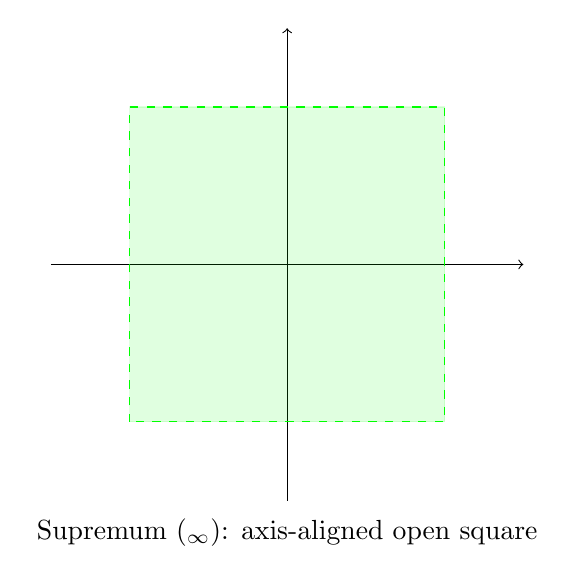
\begin{tikzpicture}[scale=1]
        \draw[->] (-3,0) -- (3,0);
        \draw[->] (0,-3) -- (0,3);
        \draw[green,fill=green,opacity=0.12] (-\r,-\r) rectangle (\r,\r);
        \draw[green,dashed] (-\r,-\r) rectangle (\r,\r);
        \node[below] at (0,-3.1) {Supremum ($\metric_\infty$): axis-aligned open square};
      \end{tikzpicture}
    \end{subfigure}

    \caption{Open balls of radius $r$ around the origin in $\R^2$ for the three metrics.}
    \label{fig:balls_1}
  \end{figure}

  Graphing these three shapes, we get Figure~\ref{fig:balls_1}.
\end{solution}

\begin{solution}[ii]
  Take the Euclidean metric $\metric_2$. Assume that $(x_n, y_n) \to (x, y)$ in the Euclidean metric. Let $\epsilon > 0$ be arbitrary. Choose $N \in \N$ such that for all $n \ge N$, $\metric_2((x_n, y_n), (x, y)) < \epsilon$. Notice that for all $n \ge N$, we have
  \[%
    |x_n - x| \le \sqrt{(x_n - x)^2 + (y_n - y)^2} = \metric_2((x_n, y_n), (x, y)) < \epsilon
  ,\]%
  and similarly $|y_n - y| < \epsilon$. Hence, $x_n \to x$ and $y_n \to y$ separately.

  For the converse, assume that $x_n \to x$ and $y_n \to y$. Let $\epsilon > 0$ be arbitrary. Choose $N = \max(\{N_1, N_2\})$, where $N_1, N_2 \in \N$ are such that for all $n \ge N_1$, $|x_n - x| < \epsilon/\sqrt{2}$ and for all $n \ge N_2$, $|y_n - y| < \epsilon/\sqrt{2}$. Then, for all $n \ge N$,
  \[%
    \metric_2((x_n, y_n), (x, y)) = \sqrt{(x_n - x)^2 + (y_n - y)^2} < \sqrt{\frac{\epsilon^2}{2} + \frac{\epsilon^2}{2}} = \epsilon
  .\]%
  Hence, $(x_n, y_n) \to (x, y)$ in the Euclidean metric.

  Therefore, a sequence $(x_n, y_n)$ converges to $(x, y)$ in the Euclidean metric if and only if $x_n \to x$ and $y_n \to y$ separately.
\end{solution}

\begin{solution}[iii]
  Clearly, $\metric(\x, \y)$ satisfies the first property of a metric. However, it fails the second identity, since if two points agree in at least one coordinate, then $\metric(\x, \y) = 0$ even if $\x \neq \y$. For example,
  \[%
    \metric((0, 0), (0, 1)) = \min\{|0 - 0|, |0 - 1|\} = 0
  ,\]%
  although $(0, 0) \neq (0, 1)$. Thus $\metric$ is not a metric on $\R^n$.
\end{solution}

\begin{problem}[1.3]
  Consider the following silly metric on $\R^2$:
  \[%
    \metric((x_1,y_1), (x_2, y_2)) = \begin{cases}
      |y_1 - y_2| & \text{if}~x_1 = x_2 \\
      |y_1 - y_2| + 1 & \text{if}~x_1 \neq x_2 \\
    \end{cases}
  .\]%
  \begin{enumerate}
    \item Prove that $\metric$ is a metric, that is, it has the three properties listed in Definition 1.2.

    \item Sketch the open balls of radius $1/2$, $1$, and $2$ around the origin in this metric.

    \item Give an example of a sequence that converges in the Euclidean metric $\metric_2$ but not in our silly metric $\metric$.

    \item Prove that every sequence that converges in $\metric$ also converges $\metric_2$.
  \end{enumerate}
\end{problem}

\begin{solution}[i]
  Clearly, $\metric((x_1, y_1), (x_2, y_2)) = \metric((x_2, y_2), (x_1, y_1))$. Also $\metric((x_1, y_1), (x_2, y_2)) = 0$ if and only if $(x_1, y_1) = (x_2, y_2)$.

  Let $(x_1, y_1), (x_2, y_2), (x_3, y_3) \in \R^2$. For the triangle inequality, observe that we may write
  \[%
    \metric((x_i, y_i), (x_j, y_j)) = |y_i - y_j| + \delta_{x_i}^{x_j}
  ,\]%
  where $\delta_a^b$ is the indicator function that is $0$ if $a = b$ and $1$ if $a \neq b$. The usual triangle inequality in $\R$ gives $|y_1 - y_3| \le |y_1 - y_2| + |y_2 - y_3|$, and the indicator satisfies
  \[%
    \delta_{x_1}^{x_3} \le \delta_{x_1}^{x_2} + \delta_{x_2}^{x_3}
  .\]%
  Adding these inequalities yields
  \[%
    \metric((x_1,y_1),(x_3,y_3)) \le \metric((x_1, y_1), (x_2, y_2)) + \metric((x_2, y_2), (x_3, y_3))
  ,\]%
  so the triangle inequality holds. Therefore $\metric$ is a metric on $\R^2$.
\end{solution}

\begin{solution}[ii]
  In this metric, points with the same $x$-coordinate have distance $|y_1 - y_2|$, while points with different $x$-coordinates have distance $|y_1-y_2|+1$. Hence, for any $r > 0$,
  \[%
    B_\metric((0, 0), r) = \{(0,y) \mid x = 0~\text{and}~|y| < r\} \,\cup\, \{(x,y) \mid x \neq 0~\text{and}~|y| < r - 1\}
  .\]%
  The second set is empty if $r \le 1$. Thus:
  \begin{align*}
    B_\metric((0, 0), 1/2) &= \{(0,y) \mid x = 0~\text{and}~|y| < 1/2\} \\
    B_\metric((0, 0), 1) &= \{(0,y) \mid x = 0~\text{and}~|y| < 1\} \\
    B_\metric((0, 0), 2) &= \{(0,y) \mid x = 0~\text{and}~|y| < 2\} \cup \{(x,y) \mid x \neq 0~\text{and}~|y| < 1\}
  .\end{align*}

  \begin{figure}[h]
    \centering

    \begin{subfigure}[b]{0.45\textwidth}
      \centering

      % Ball of radius 1/2
      \begin{tikzpicture}[scale=1.0]
        \draw[->] (-2,0) -- (2,0) node[right] {$x$};
        \draw[->] (0,-2) -- (0,2) node[above] {$y$};
        % Ball of radius 1/2: vertical line segment along x=0
        \draw[very thick,blue] (0,-0.5) -- (0,0.5);
      \end{tikzpicture}

      \caption{Radius $1/2$}
    \end{subfigure}
    \begin{subfigure}[b]{0.45\textwidth}
      \centering

      \begin{tikzpicture}[scale=1.0]
        \draw[->] (-2,0) -- (2,0) node[right] {$x$};
        \draw[->] (0,-2) -- (0,2) node[above] {$y$};
        % Ball of radius 1: vertical line segment along x=0
        \draw[very thick,blue] (0,-1) -- (0,1);
      \end{tikzpicture}

      \caption{Radius $1$}
    \end{subfigure}

    \begin{subfigure}[b]{0.45\textwidth}
      \centering

      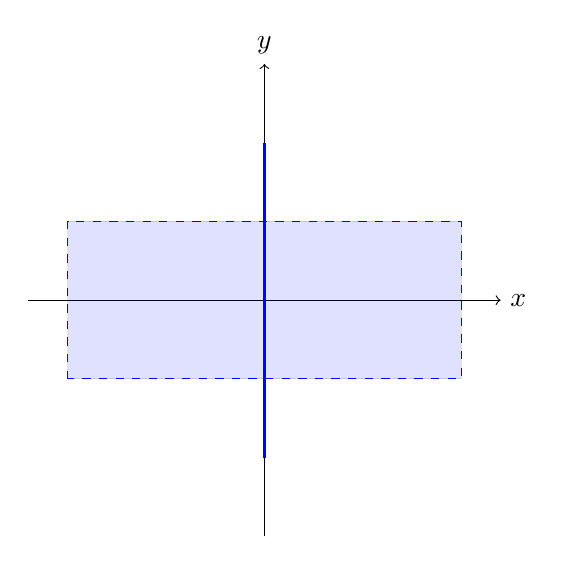
\begin{tikzpicture}[scale=1.0]
        \draw[->] (-3,0) -- (3,0) node[right] {$x$};
        \draw[->] (0,-3) -- (0,3) node[above] {$y$};
        % Part on x=0: vertical line segment from -2 to 2
        \draw[very thick,blue] (0,-2) -- (0,2);
        % For all x != 0: vertical line segments from -1 to 1
        \draw[fill=blue,opacity=0.12] (-2.5,-1) rectangle (2.5,1);
        \draw[blue,dashed] (-2.5,-1) rectangle (2.5,1);
      \end{tikzpicture}

      \caption{Radius $2$}
    \end{subfigure}

    \caption{}
    \label{fig:balls_2}
  \end{figure}

  Graphing these three shapes, we get Figure~\ref{fig:balls_2}.
\end{solution}

\begin{solution}[iii]
  Take $(a_n) = (1/n, 0)$. Then $(a_n)$ converges to $(0, 0)$ in the Euclidean metric $\metric_2$ since
  \[%
    \metric_2(a_n, (0, 0)) = \sqrt{(1/n - 0)^2 + (0 - 0)^2} = 1/n \to 0
  .\]%
  But in the silly metric $\metric$, we have
  \[%
    \metric(a_n, (0, 0)) = |0 - 0| + 1 = 1 \not\to 0
  .\]%
  Hence, $(a_n)$ does not converge to $(0, 0)$ in the silly metric.
\end{solution}

\begin{solution}[iv]
  Let $(a_n) = (x_n, y_n)$ converge to $a = (x, y)$ in the metric d, so $\metric(a_n, a) \to 0$. Choose $\epsilon = 1/2$. Then, there exists $N_1 \in \N$ such that for all $n \ge N_1$, $\metric(a_n, a) < 1/2$. But if $x_n \ne x$ then $\metric(a_n, a) = |y_n - y| + 1 \ge 1$, contradiction. Hence $x_n = x$ for all $n \ge N_1$.

  Now, let $\epsilon > 0$ be arbitrary. Since $\metric(a_n, a) \to 0$, there exists $N_2 \in \N$ such that for all $n \ge N_2$, $\metric(a_n, a) < \epsilon$. For $n \ge N \coloneqq \max(\{N_1, N_2\})$, we have $x_n = x$ and so $\metric(a_n, a) = |y_n - y| < ε$. Hence, for $n \ge N$,
  \[%
    \metric_2(a_n, a) = \sqrt{(x_n - x)^2 + (y_n - y)^2} = |y_n - y| < \epsilon
  .\]%
  Therefore $\metric_2(a_n, a) \to 0$, and $(a_n)$ converges to $a$ in the Euclidean metric.
\end{solution}

\begin{problem}[1.4]
  Let $X$ be any set, and let $\metric_X$ be the \emph{discrete metric}
  \[%
    \metric_X(p, q) = \begin{cases}
      0 & \text{if}~p = q \\
      1 & \text{if}~p \neq q \\
    \end{cases}
  .\]%
  \begin{enumerate}
    \item Prove that $\metric_X$ is a metric

    \item Let $(Y, \metric_Y)$ be another metric space (not necessarily discrete). Prove that every map $f : X \to Y$ is continuous.

    \item Prove that a sequence $p_1, p_2, p_3, \cdots \in X$ converges in the discrete metric if and only if it is eventually constant.
  \end{enumerate}
\end{problem}

\begin{solution}[i]
  Clearly, $\metric_X(p, q) = \metric_X(q, p)$ for all $p, q \in X$. Also, $\metric_X(p, q) = 0$ if and only if $p = q$. We now prove that the metric satisfies the triangle inequality. Let $p, q, r \in X$. If any two of the points are equal, then the triangle inequality hold trivially. So, assume that $p, q, r$ are all distinct. Then,
  \[%
    \metric_X(p, r) = 1 \le \metric_X(p, q) + \metric_X(q, r) = 1 + 1 = 2
  .\]%
  Thus, $\metric_X$ is a metric on $X$.
\end{solution}

\begin{solution}[ii]
  Let $p \in X$ and $\epsilon > 0$. Choose $\delta = 1/2$. Then $B(p,\delta) = \{p\}$. Thus, if $q \in B(p,\delta)$, we must have $q = p$, and so
  \[%
    d_Y(f(p), f(q)) = d_Y(f(p), f(p)) = 0 < \epsilon
  .\]%
  Hence $f$ is continuous at $p$. Since $p \in X$ was arbitrary, $f$ is continuous on $X$. 
\end{solution}

\begin{solution}[iii]
  Assume that the sequence $(p_n) = (p_1, p_2, p_3, \dots)$ converges to $p \in X$. By definition, for every $\epsilon > 0$, there exists $N \in \N$ such that for all $n \geq N$, $\metric_X(p_n, p) < \epsilon$. Choose $\epsilon = 1/2$. Then, for all $n \geq N$, $\metric_X(p_n, p) < 1/2$. Since the distance between any two distinct points in $X$ is $1$, this implies that $p_n = p$ for all $n \geq N$. Thus, the sequence is eventually constant.

  Conversely, assume that the sequence $(p_n)$ is eventually constant. Then there exists $N \in \N$ and $p \in X$ such that $p_n = p$ for all $n \geq N$. Let $\epsilon > 0$ be arbitrary. For this $N$, we have $\metric_X(p_n, p) = 0 < \epsilon$ whenever $n \geq N$. Hence, by definition, $(p_n)$ converges to $p$.
\end{solution}

\begin{problem}[1.11]
  Let $(X, \metric_X)$ and $(Y, \metric_Y)$ be metric spaces, let $(p_n) = (p_1, p_2, p_3, \cdots)$ be a sequence that converges to a point $\ell$ in $X$, and let $f : X \to Y$ be continuous at $\ell$. Prove that the sequence $f(p_n) = f(p_1), f(p_2), f(p_3), \cdots$ converges to $f(\ell)$ in $Y$.
\end{problem}

\begin{solution}
  Since $f$ is continuous at $\ell$ (since $\ell \in X$), for every $\epsilon > 0$, there exists $\delta > 0$ such that for all $x \in X$ with $\metric_X(x, \ell) < \delta$, we have $\metric_Y(f(x), f(\ell)) < \epsilon$. Since $(p_n)$ converges to $\ell$, for this $\delta > 0$, there exists $N \in \N$ such that for all $n \geq N$, $\metric_X(p_n, \ell) < \delta$. Therefore, for all $n \geq N$, we have $\metric_Y(f(p_n), f(\ell)) < \epsilon$. This shows that the sequence $(f(p_n))$ converges to $f(\ell)$ in $Y$.
\end{solution}
